\documentclass{beamer}
\usepackage[utf8]{inputenc}
\usepackage{caption}

\usetheme{Copenhagen}
%color themes: default, beaver, beetle, seahorse, wolverine
\usecolortheme{default}
 
 
%Information to be included in the title page:
\title{Bastion The Sentinel}
\author{Park Cleaner Robot}
\institute{Istanbul Bilgi University}
\date{\today}
 
 
\begin{document}
 % Giriş sayfasını yazdır
 \frame{\titlepage}
 
 %scope slaytı
 \begin{frame}
  \frametitle{SCOPE}
  \begin{itemize}
   \item Consuming essential for humans
   \item It leads to pollution
   \item Our main goal is separating and recycling the garbages
  \end{itemize}
 \end{frame}

 %device functionality slaytı
 \begin{frame}
  \frametitle{DEVICE FUNCTIONALITY}
  \begin{itemize}
   \item Bastion The Sentinel will be a multi-tasking that has three main parts.
   \begin{itemize}
    \item Movement controls
    \item Robotic arm controls
    \item Camera
   \end{itemize}
   \item Robotic arm uses image processing to collect garbages
   \begin{itemize}
    \item Image recognization by color difference
   \end{itemize}
   \item Operator takes control in emergency situations
  \end{itemize}
 \end{frame}

 %device functionality slaytı
 \begin{frame}
  \frametitle{DEVICE FUNCTIONALITY}
  \begin{itemize}
   \item It has a box for collecting garbages.
   \item It has 6 wheels. 
   \item It uses a camera to detect objects.
  \end{itemize}
 \end{frame}

 %overall design scheme
 \begin{frame}
  \frametitle{OVERALL DESIGN SCHEME}
  \begin{figure}[h]
   \begin{center}
    \includegraphics[scale=0.6]{block_diagram}
    \caption{Block diagram of the system}
   \end{center}
  \end{figure}
 \end{frame}
 
 %details of design
 \begin{frame}
  \frametitle{DESIGN AND DETAILS}
  \begin{itemize}
   \item Input Block
   \begin{itemize}
    \item Camera Sensor
    \item Serial Input
   \end{itemize}
   \item Control Block
   \item Output Block
   \item Communication Block
  \end{itemize}
 \end{frame}

 %input block
 \begin{frame}
  \frametitle{Input Block}
  \begin{itemize}
    \item Raspberry Pi transfers the video data to client over the WIFI.
    \item On the client side image processing performed by using OpenCV library.
    \item Detecting garbages by their color range.
    \item Raspberry and Arduino connected as master-slave.
    \item Raspberry manages the serial connection on Arduino.
  \end{itemize}
 \end{frame}
 
 %control block
 \begin{frame}
  \frametitle{Control Block}
  \begin{flushleft}
     \begin{figure}[h!]
      \begin{center}
       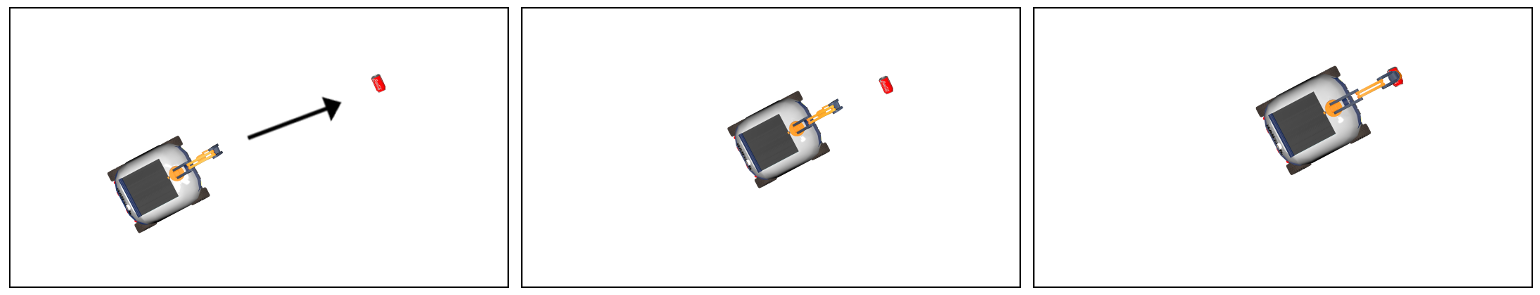
\includegraphics[scale=0.2]{3frame}
       \caption{\textbf{Bastion The Sentinel} is approaching to an object.}
      \end{center}
     \end{figure}
     Raspberry Pi will manage the Arduino to use the motor shields. 
    \end{flushleft}
 \end{frame}

 % output block
 \begin{frame}
  \frametitle{Output Block}
  \begin{itemize}
   \item Raspberry Pi is in charge of controlling the Arduino.
   \item Aurdino is connected to the motor shields and the robotic arm.
   \item Bastion The Sentinel has two different speed choice. Slow for fine adjustments and fast 
   for quick jobs.
   \item Robotic arm has 3 joints and has 1 gripper.
   \item Arm can rotate 360$^{\circ}$ and it can be collapsed to minimize the area.
   \item Also gripper part will have the ability to rotate up to 180$^{\circ}$.
  \end{itemize}
 \end{frame}
 
 %communication block
 \begin{frame}
  \frametitle{Communication Block}
  \begin{itemize}
   \item Serial connection over the WIFI.
   \item Real time video data will be gathered on the robot and will be sent to client.
   \item Video data will be processed on the client side.
   \item Simultaneous data transmission.
  \end{itemize}
 \end{frame}
 
  %communication block
 \begin{frame}
  \frametitle{Communication Block}
  \begin{figure}[h!]
    \begin{center}
      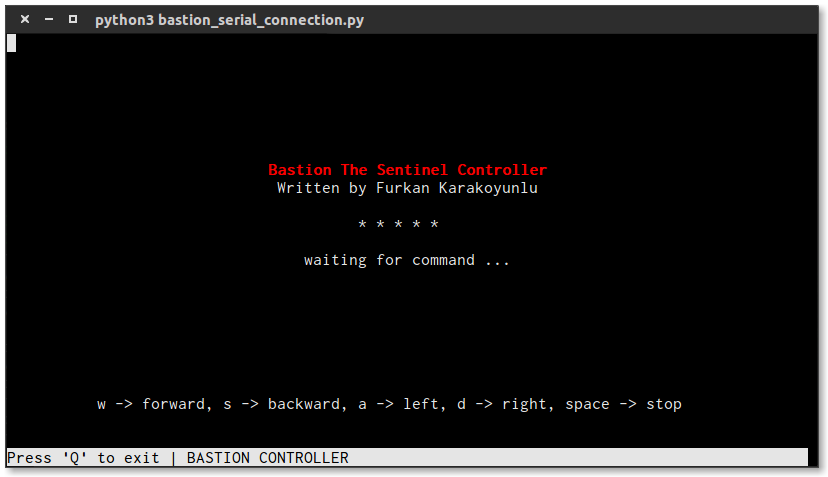
\includegraphics[scale=0.35]{serial_pc}
      \caption{Serial connection screen from PC}
    \end{center}
  \end{figure}
 \end{frame}
 
   %communication block
 \begin{frame}
  \frametitle{Communication Block}
  \begin{figure}[h!]
    \begin{center}
      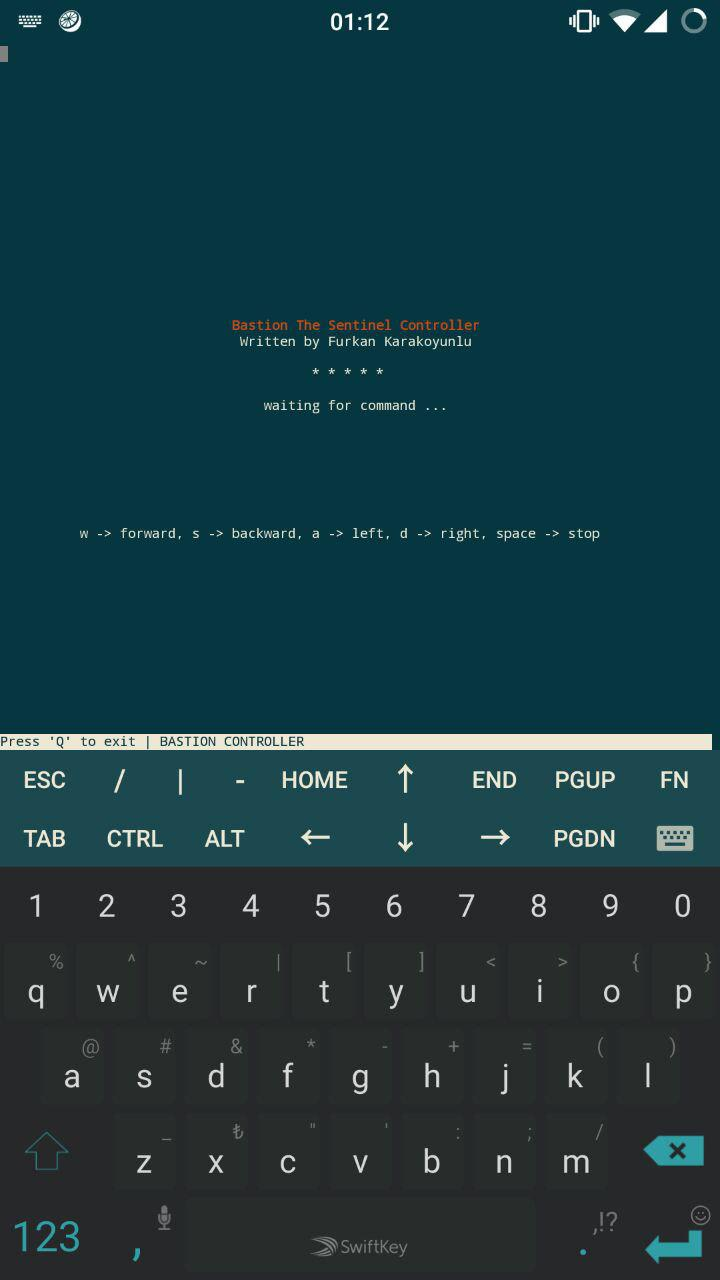
\includegraphics[scale=0.15]{serial_phone}
      \caption{Serial connection screen from smart phone}
    \end{center}
  \end{figure}
 \end{frame}
 
   %image processing
 \begin{frame}
  \frametitle{Image Processing}
  \begin{figure}[h!]
    \begin{center}
      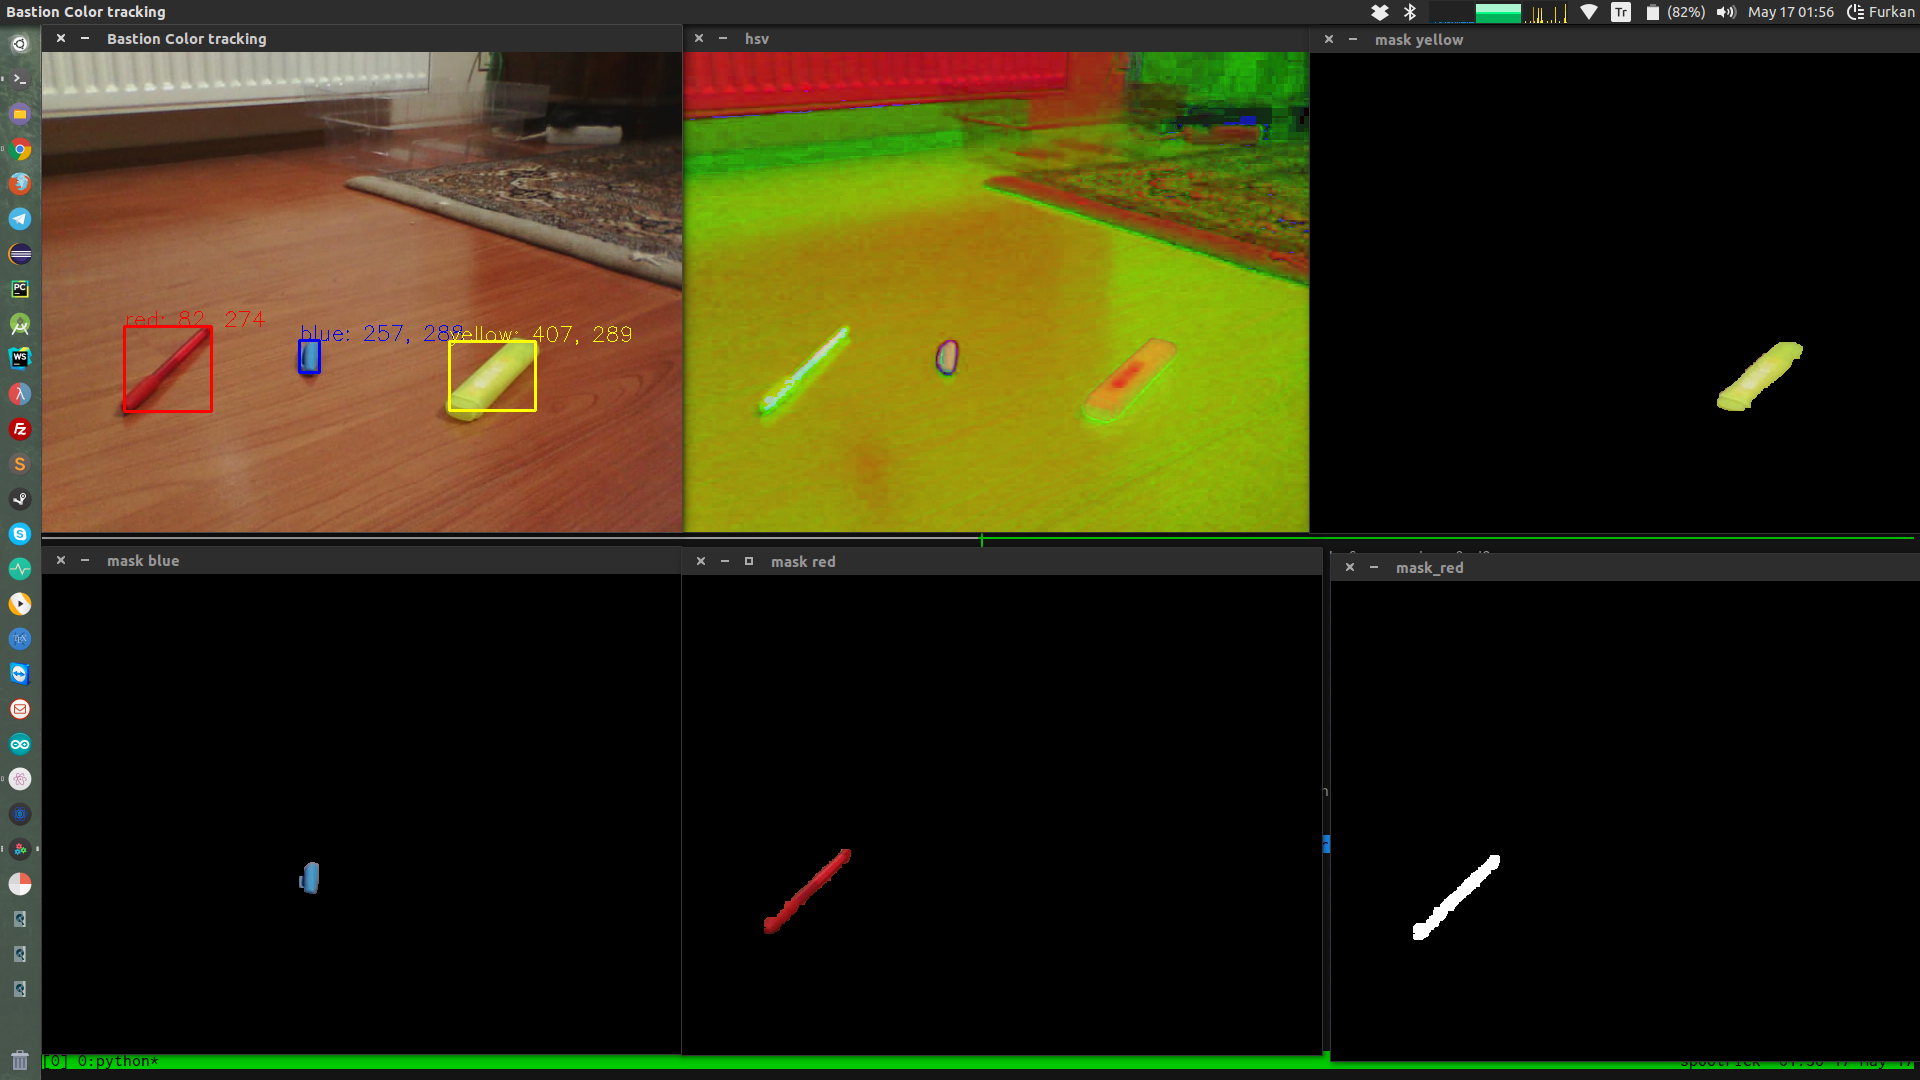
\includegraphics[scale=0.15]{opencv_python}
      \caption{Image processing screen on the client.}
    \end{center}
  \end{figure}
 \end{frame}
 
  %budget
 \begin{frame}
  \frametitle{BUDGET}
  \begin{center}
   \begin{tabular}{|l|r|}
   \hline
   \bf Item & \bf Price(TL)\\
   \hline
   Dagu Wild Thumper 6WD All-Terrain Chassis & 1.363,88\\
   VNH5019 Motor Driver & 212,70\\
   7,4 Volt 4000 mAh LiPo Battery & 149,72\\
   Battery charger unit & 195,39\\
   3D Printed Robotic Arm & 400,00\\
   Arduino Mega & 181,48\\
   Raspberry Pi 3 Model B & 190,86\\
   2 x Raspberry Pi Camera Module & 113,00\\
   8 x Servo Motor & 228,00\\
   Tools & 87,23\\
   \hline
   \bf Total & \bf 3122,26\\
   \hline
   \end{tabular}
   \captionof{table}{Budget for building the robot}
  \end{center}

 \end{frame}

 %Business plan
 \begin{frame}
  \frametitle{BUSINESS PLAN}
  \begin{itemize}
   \item In Turkey, pollution rates are higher than other countries
   \item There is no proper way to solve this problem
   \item The purpose of creating this robot is to protect the nature and speed up the recycling process
   \item It takes so many years for some materials to dissolve in nature
   \item \%75 of garbages are recyclable but \%30 percent of it used used in recycling process
   \item Someone should step up and do something about it
   \item While we are making the nature cleaner, also we are aiming to build a robot which has recyclable parts as much as possible.
  \end{itemize}
 \end{frame}
 
 \begin{frame}
  Demonstration
 \end{frame}
 
  \begin{frame}
  Thank you for listening.\\
  \bigskip
  Furkan Karakoyunlu\\
  112200036
 \end{frame}
\end{document}